\documentclass[a4paper,10pt]{article}
\newcommand{\path}{../../../../../mygit/_Latex/}
\input{\path StdPack.tex}
\usepackage{\path cmds}
\newcommand{\bibTitle}[1]{``#1''}
\graphicspath{{figures/}}
\begin{document}



\section{Application to linear array}\label{section:linearArray}


This section explores the effect of multiple scattering on the elementary case of a linear array of identical
circularly symmetric scattering bodies.
For simplicity, the simulations are performed in 2D but the general conclusions should equally apply to 3D
simulations.

The interlattice distance, the strength of the potential and the number of scattering elements, i.e. the thickness
of the sample are allowed to vary.
The potential profile is Gaussian as shown in figure~\ref{fig:singleArrayV}.
% is either constant over the circular element or  .
The wavelength is kept at 200keV for all the simulations, the radius being about $1A$ resulting in a
normalized radius $ka\approx 2\pi/\lambda r_0\approx 250$.



\begin{figure}[h!]
	\begin{subfigure}{0.45\textwidth}
		\centering
		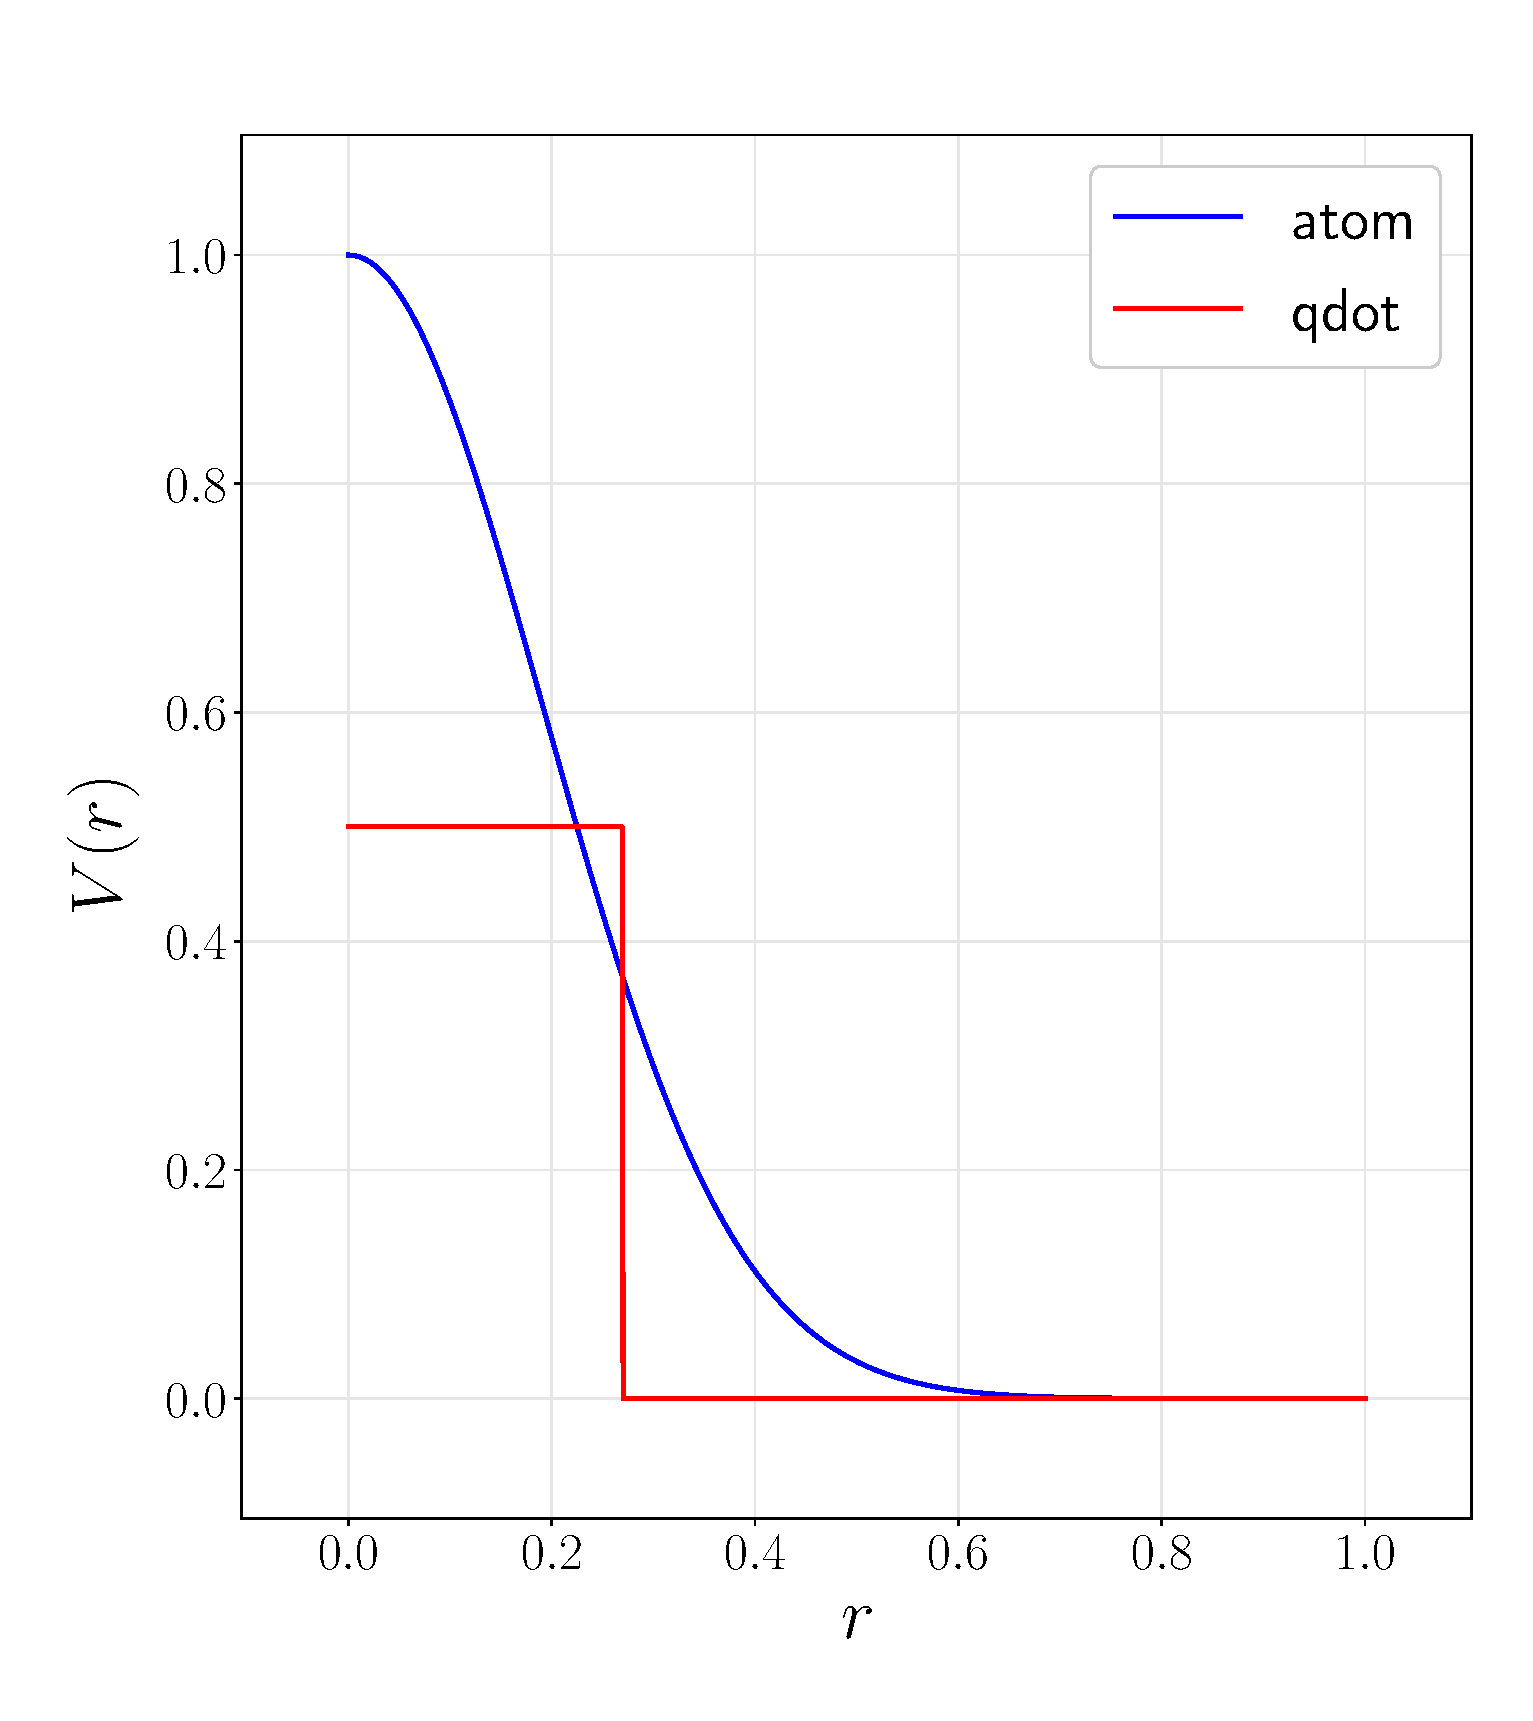
\includegraphics[width=\textwidth]{figures/potential.eps}
		\caption{}\label{fig:singleArrayV}
	\end{subfigure}
	\begin{subfigure}{0.45\textwidth}
		\centering
		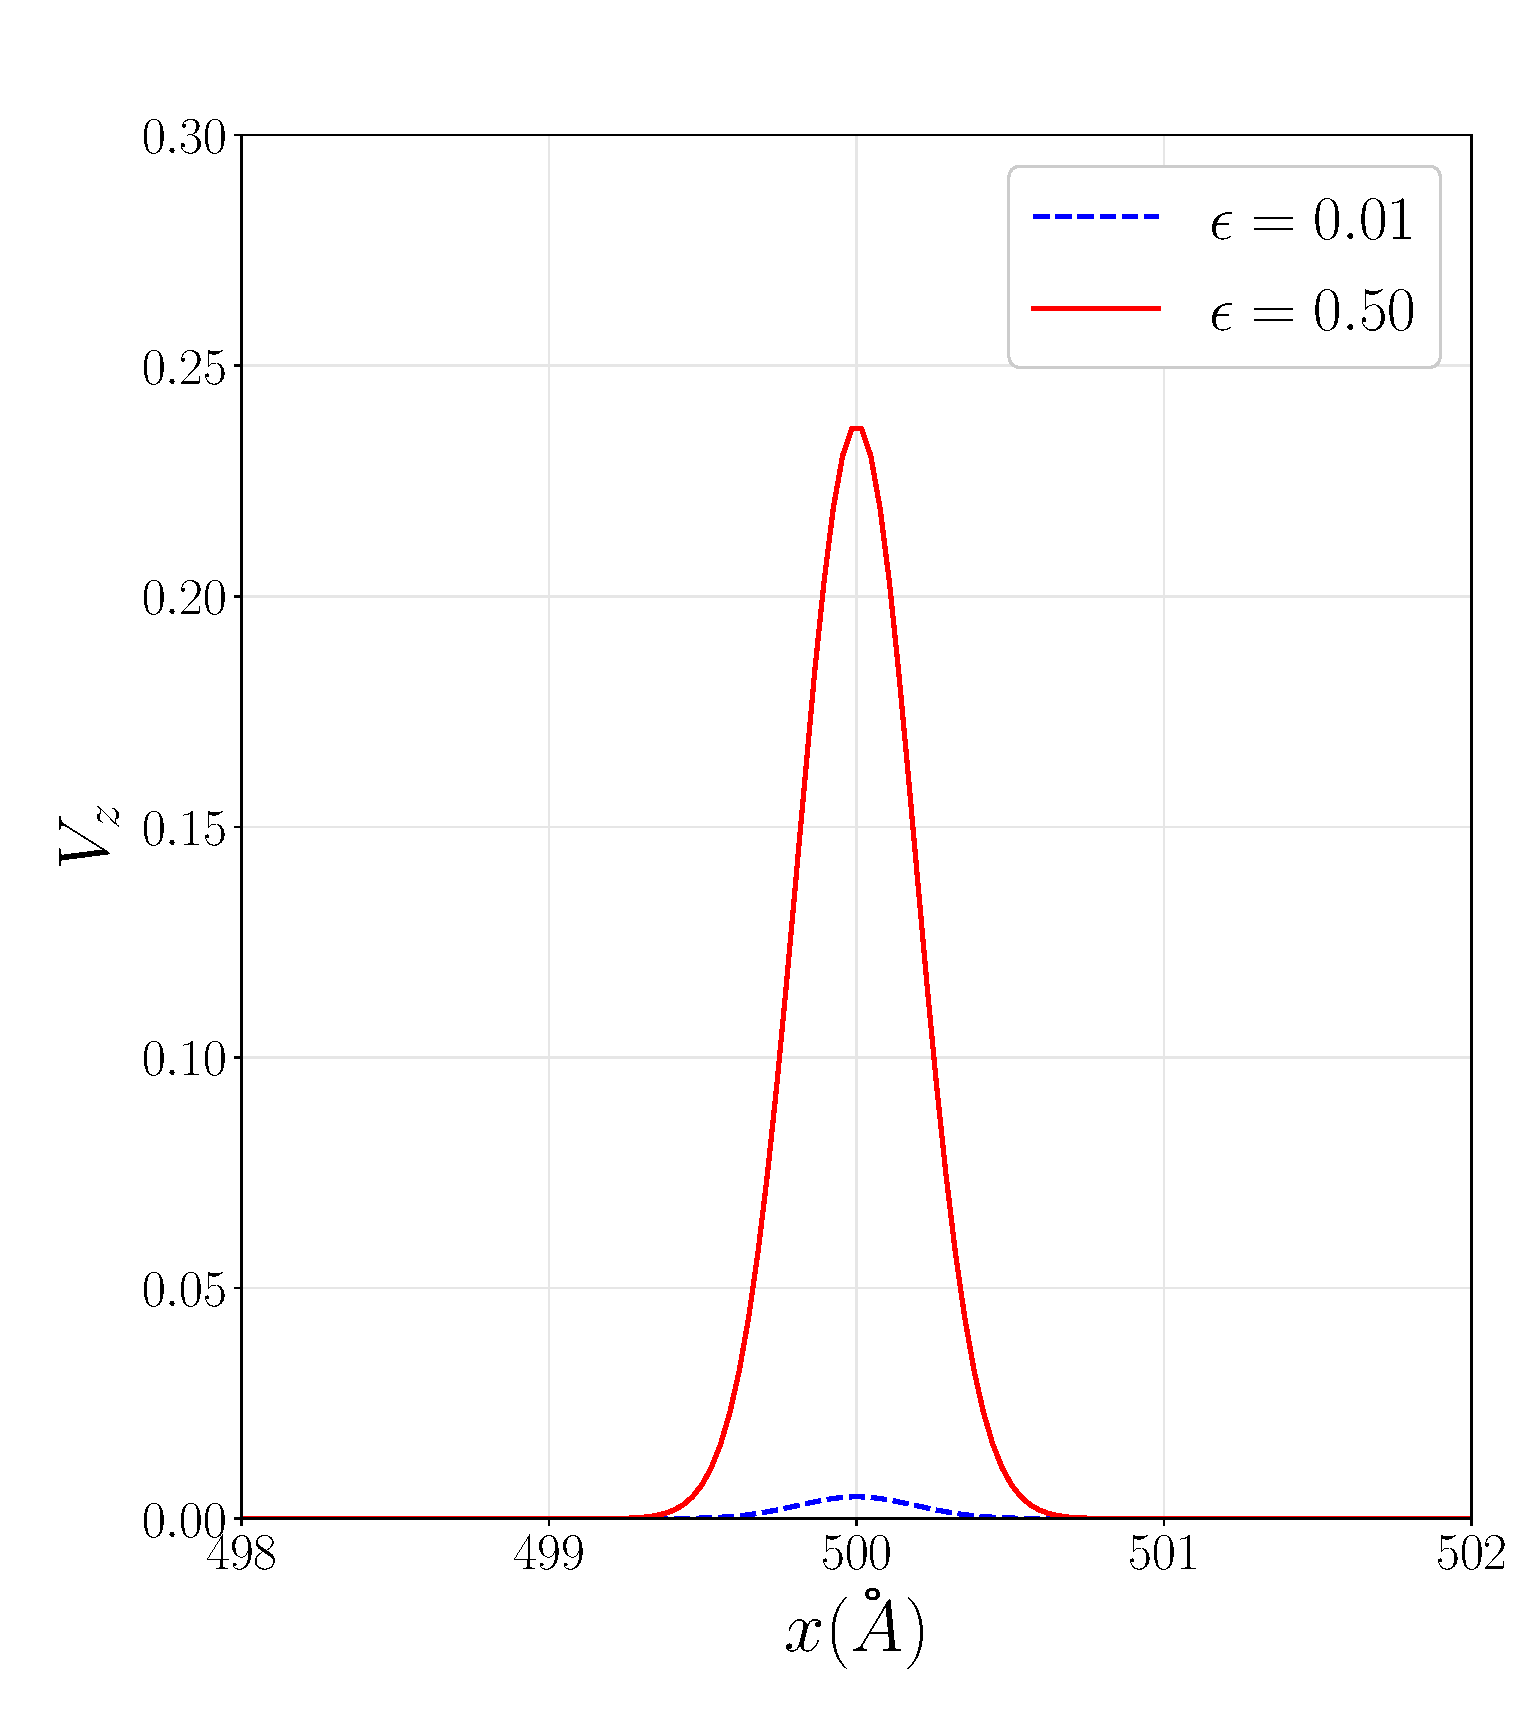
\includegraphics[width=\textwidth]{figures/projV.eps}
		\caption{}\label{fig:singleArrayVproj}
	\end{subfigure}

	\caption[single array]{
		\ref{fig:singleArrayV} Potential constant over the circular area $qdot$ and Gaussian $atom$.
		\ref{fig:singleArrayVproj} Projected potential.
	}\label{fig:singleArrayVV}
\end{figure}




\begin{figure}
	\begin{subfigure}{0.3\textwidth}
		\centering
		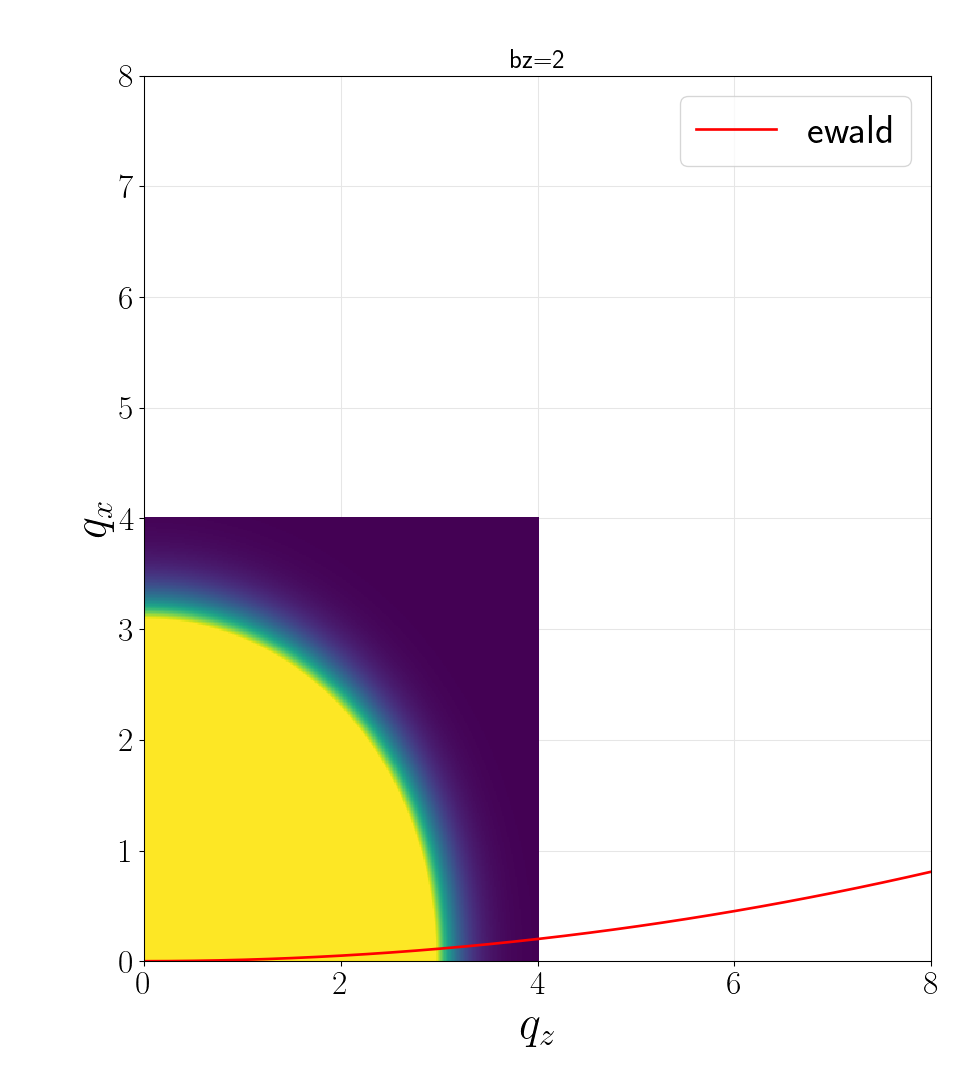
\includegraphics[width=\textwidth]{kd1_V.png}
		\caption{}\label{fig:singleArray_kd1_V}
	\end{subfigure}
	\begin{subfigure}{0.3\textwidth}
		\centering
		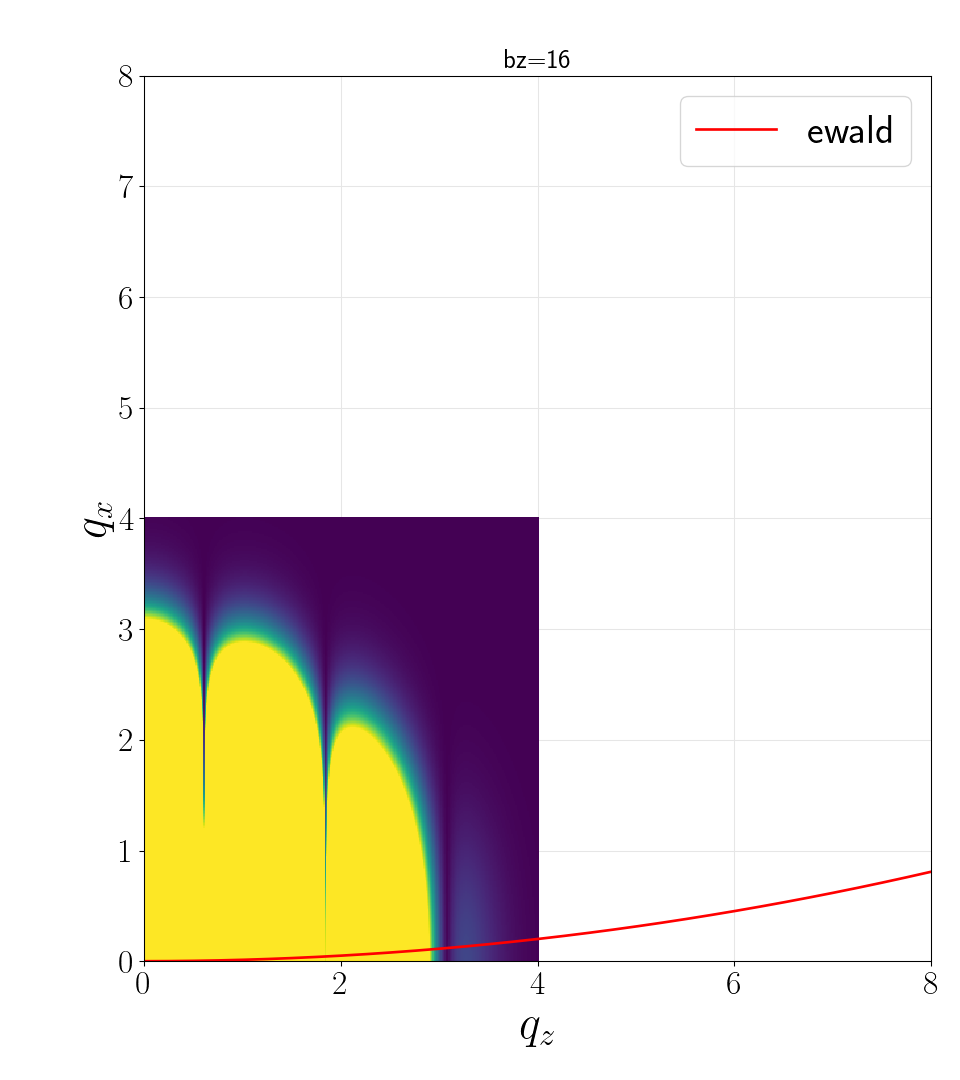
\includegraphics[width=\textwidth]{kd2_V.png}
		\caption{}\label{fig:singleArray_kd2_V}
	\end{subfigure}
	\begin{subfigure}{0.3\textwidth}
		\centering
		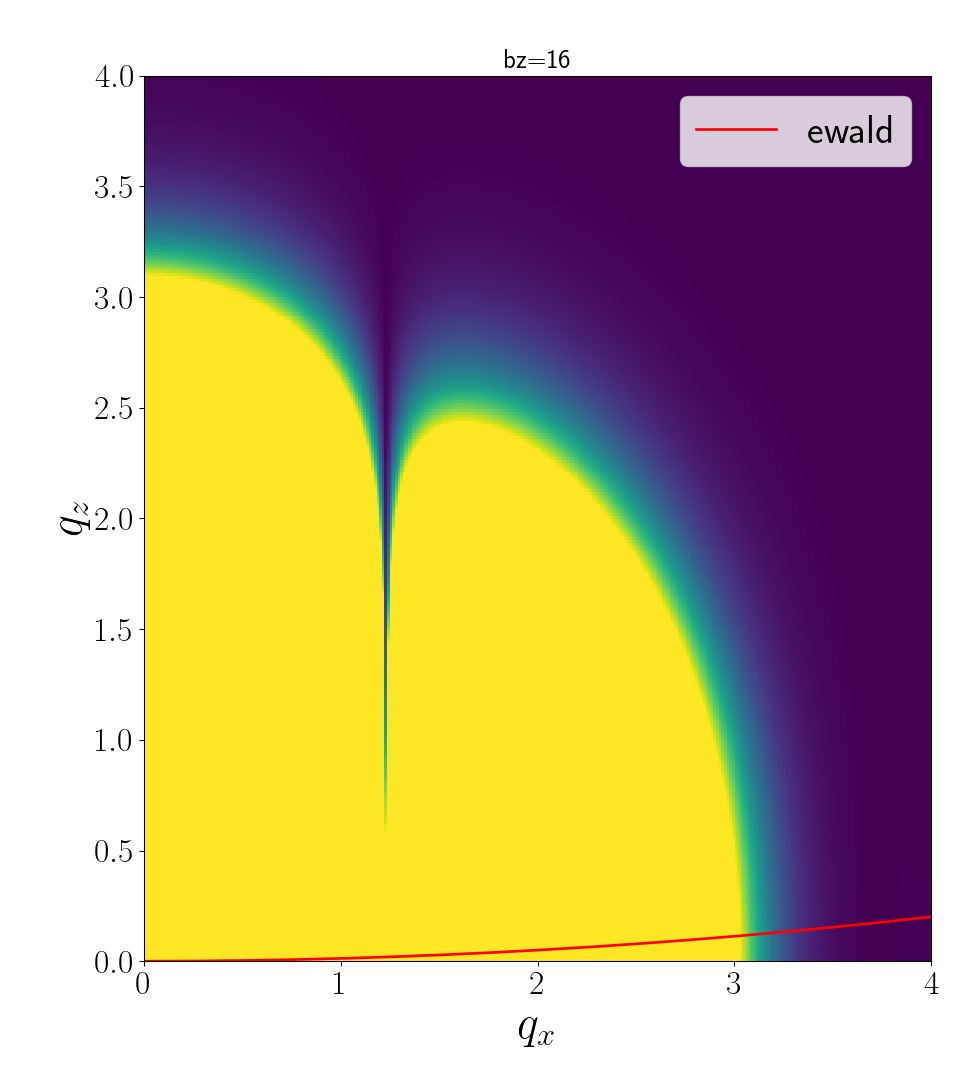
\includegraphics[width=\textwidth]{kd3_V.png}
		\caption{}\label{fig:singleArray_kd3_V}
	\end{subfigure}

	\begin{subfigure}{0.3\textwidth}
		\centering
		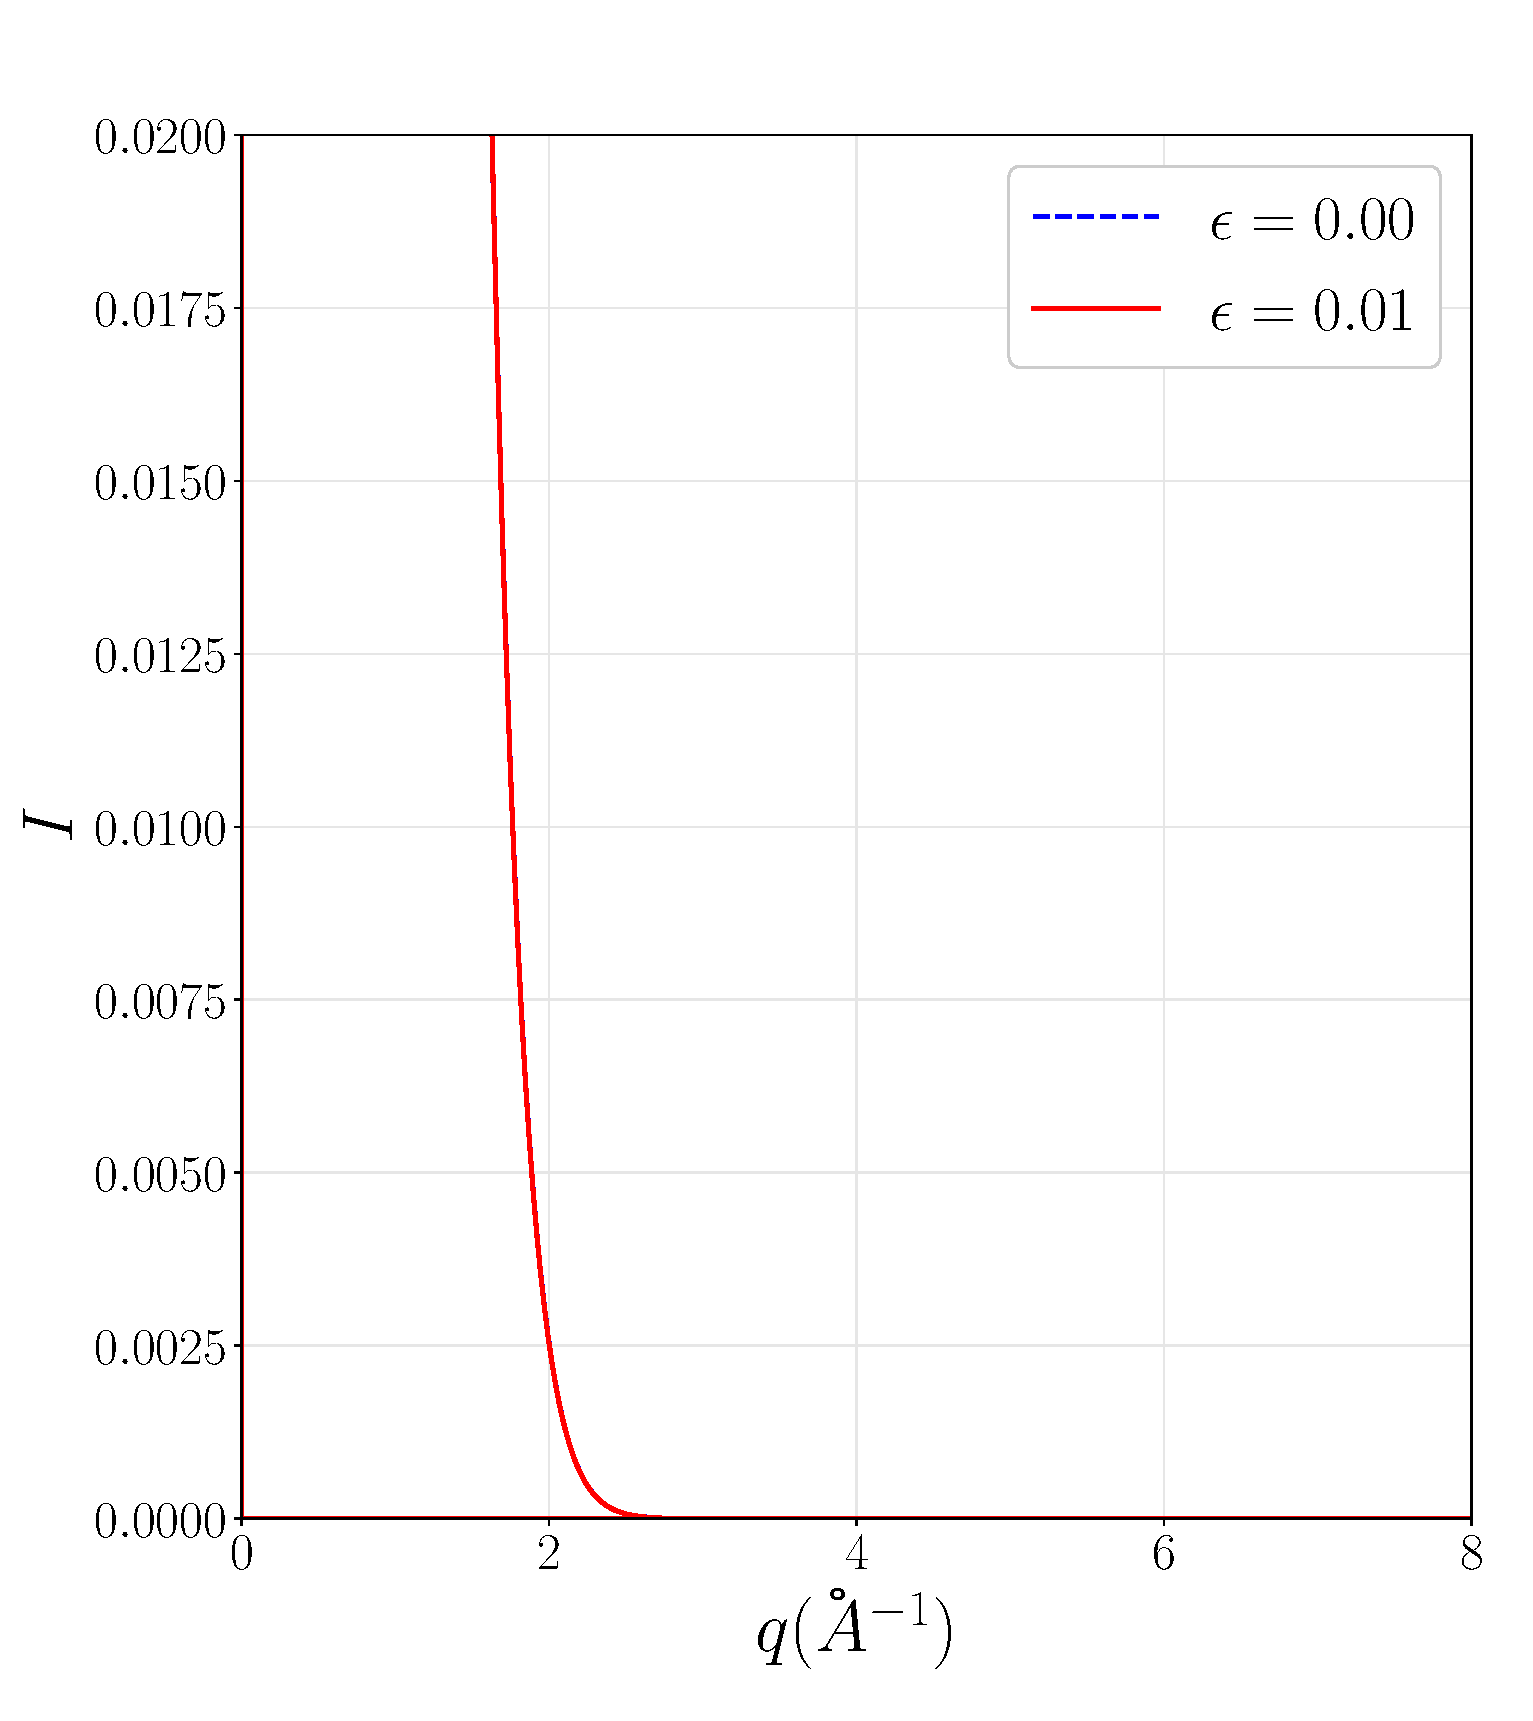
\includegraphics[width=\textwidth]{kd1_D.eps}
		\caption{}\label{fig:singleArray_kd1_D}
	\end{subfigure}
	\begin{subfigure}{0.3\textwidth}
		\centering
		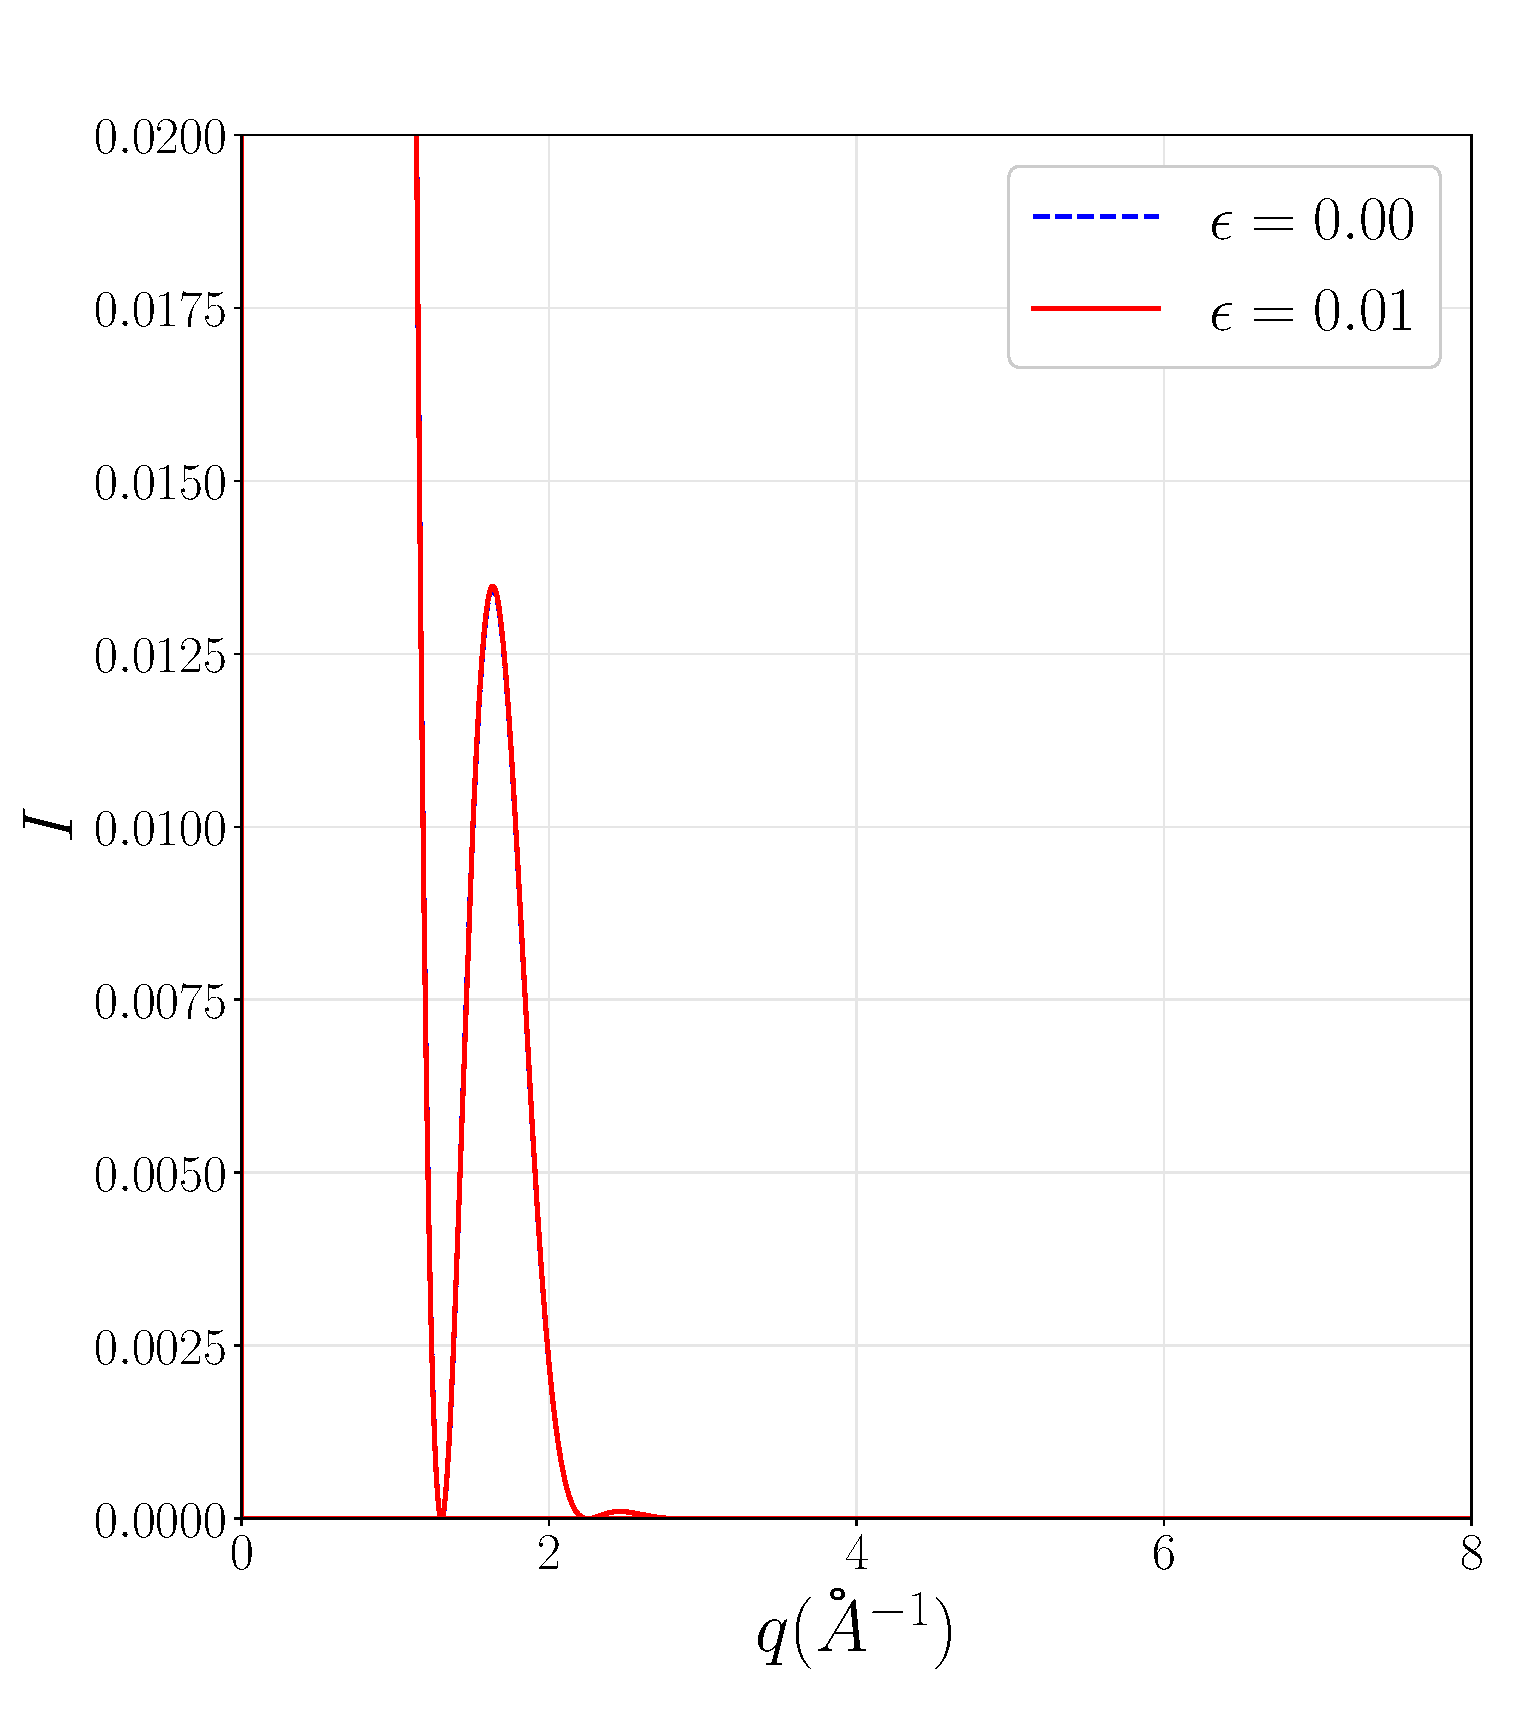
\includegraphics[width=\textwidth]{kd2_D.eps}
		\caption{}\label{fig:singleArray_kd2_D}
	\end{subfigure}
	\begin{subfigure}{0.3\textwidth}
		\centering
		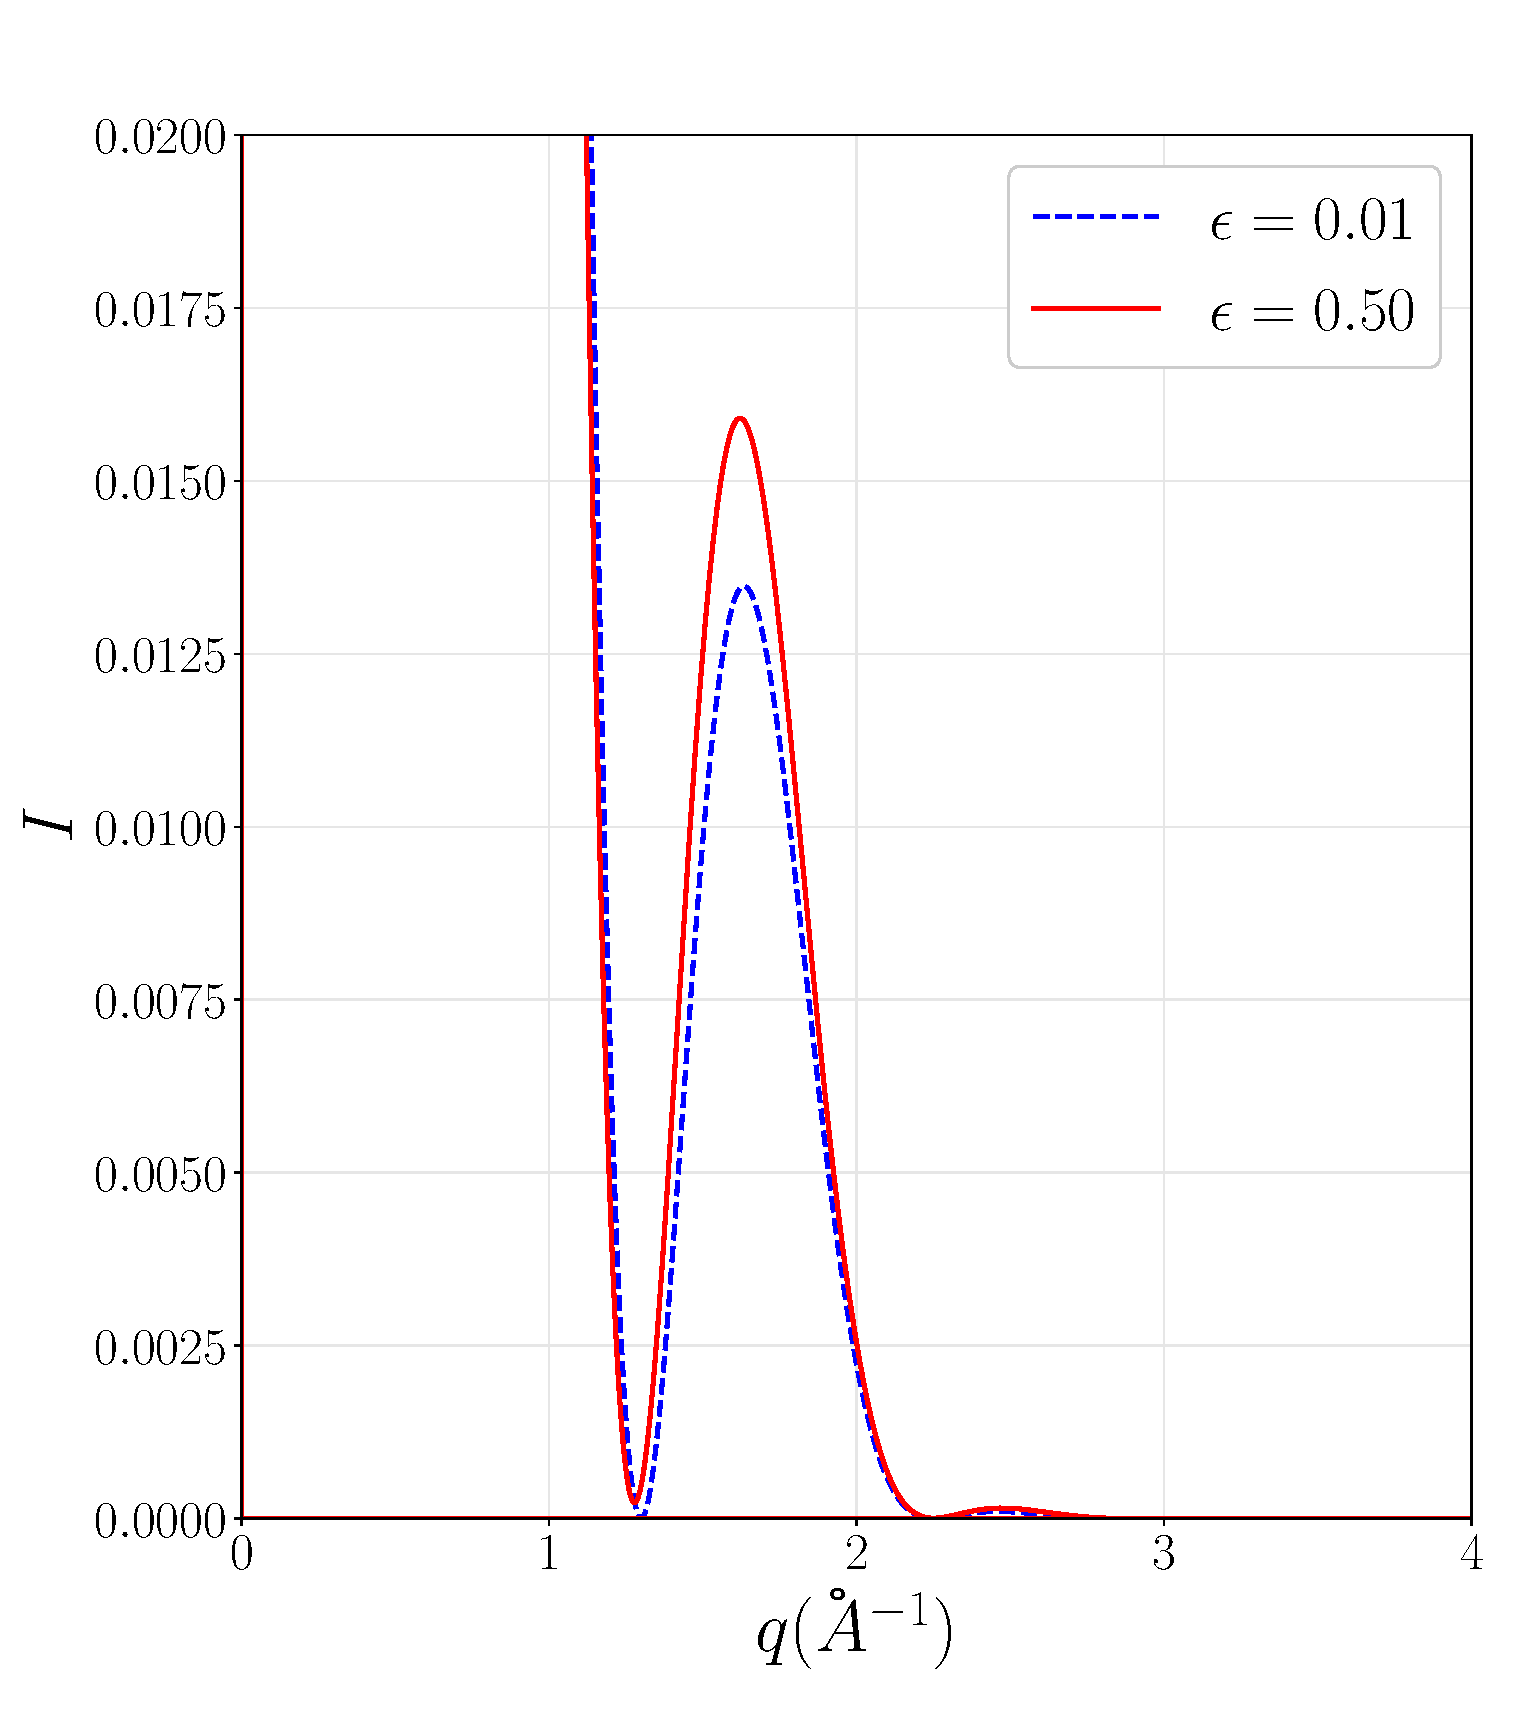
\includegraphics[width=\textwidth]{kd3_D.eps}
		\caption{}\label{fig:singleArray_kd3_D}
	\end{subfigure}

	\caption[single array interllatice distance]{
	2D Potential and diffraction pattern for a 2-scattering bodies with interlattice distance
	\ref{fig:singleArray_kd1_V},\ref{fig:singleArray_kd1_D} d=2,
	\ref{fig:singleArray_kd2_V},\ref{fig:singleArray_kd2_D} d=4,
	\ref{fig:singleArray_kd3_V},\ref{fig:singleArray_kd3_D} d=8.
	Solid lines correspond to dynamical diffraction due to strong potential and
	dashed lines for kinematic weak potential.
	}\label{fig:singleArray_kd}
\end{figure}



\end{document}
